\section{Robot Motion}
This section will seek to explain three different motion models. The velocity based motion model, the odometry based motion model and the map based motion model. The models acts as a way to determine the outcome of a movement command. It is based on a robot pose which can be seen in figure \ref{fig:robotpose}.
\begin{figure}[H]
\centering
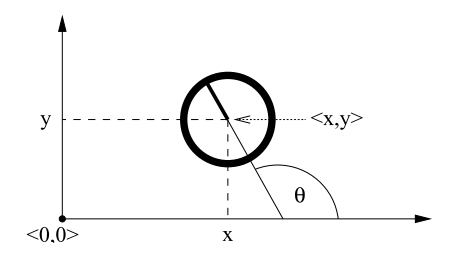
\includegraphics[width=0.8\textwidth]{billeder/robotpose}
\caption{Robot pose}
\label{fig:robotpose}
\end{figure}
The pose is defined as a vector in a 2D world:
\begin{equation}
robotpose := ( x, y, \theta ) ^T
\end{equation}
The vector has a position, $[ x, y ]$ and and an angle, $\theta$. For robots moving in more dimensions, the vector will have to be larger to accommodate the coupling between these dimensions. Only 2D cases will be explained in this section.\\

When a robot moves, the movement will not produce a perfect transition between two positions. The intrinsic noise in the movement apparatus will provide both angular noise and positional noise. This means our model will have to be probabilistic. The probability of being in position $x_t$ given a motion control command $u_t$ and a previous position is defined as in equation \ref{eq:posterior}.
\begin{equation}
p(x_t | u_t, x_{t-1})
\label{eq:posterior}
\end{equation}
An example of posterior distribution is seen in figure \ref{fig:postdist}. The figure shows that more complex movement behaviours will result in more uncertainty of where the robot is positioned when the movement ends.
\begin{figure}[H]
\centering
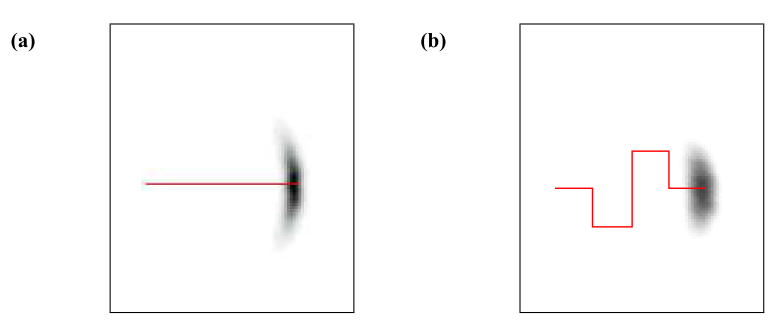
\includegraphics[width=0.8\textwidth]{billeder/postdist}
\caption{Posterior distribution}
\label{fig:postdist}
\end{figure}

\subsection{Velocity based motion model}
In the velocity based motion model, the posterior distribution is still given by equation \ref{eq:posterior}. The control command is defined as $u_t = (v_t, \omega_t )^T $. $v_t$ is the translational velocity at time t. $\omega_t$ is the rotational velocity at time t. In figure \ref{fig:velocmod} three different cases are seen. (a) is a regular case with moderate translation and rotational error. (b) is a case with large translational error and (c) is a case with large rotational error.
\begin{figure}[H]
\centering
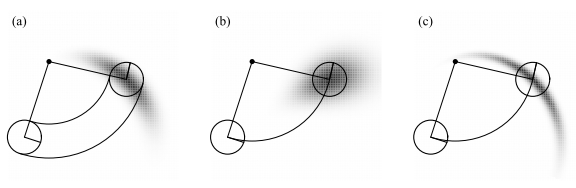
\includegraphics[width=0.8\textwidth]{billeder/velocmod}
\caption{Velocity based motion model}
\label{fig:velocmod}
\end{figure}
The algorithm for the velocity based motion model can be seen in figure \ref{fig:motionmodelalgo}. This is the algorithm behind the model seen in figure \ref{fig:velocmod} as well. The \textbf{prob} function is either normal distributed or triangular distributed. $\alpha_1$ to $\alpha_6$ determines the error introduced in our model.
\begin{figure}[H]
\centering
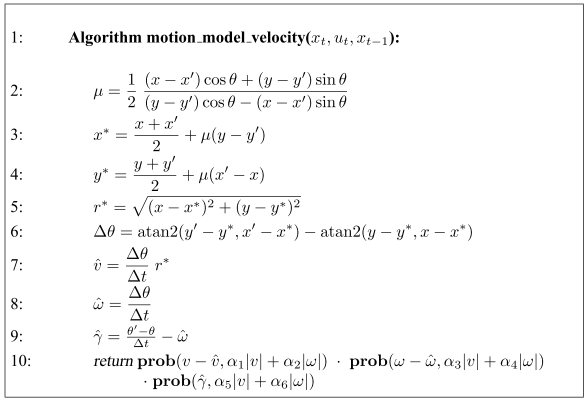
\includegraphics[width=0.8\textwidth]{billeder/motionmodelalgo}
\caption{Velocity based motion model algorithm}
\label{fig:motionmodelalgo}
\end{figure}
When executing the algorithm the outcome will be an estimated final pose. This is useful as it can be used for prediction purposes. For discrete spaces sampling velocity based motion model algorithm is used. This is seen in figure \ref{fig:samplemodelalgo}.
\begin{figure}[H]
\centering
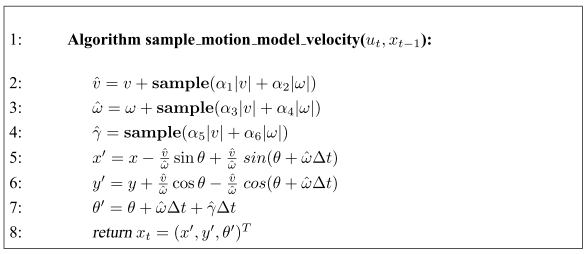
\includegraphics[width=0.8\textwidth]{billeder/samplemodelalgo}
\caption{Sampling velocity based motion model algorithm}
\label{fig:samplemodelalgo}
\end{figure}
The \textbf{sample} function returns a sample from either a normal or a triangular distribution with $\mu = 0$ and $\sigma^2$ being the input parameter. As with the non-sampling version, $\alpha_1$ to $\alpha_6$ determines the error introduced in our model.
\subsection{Odometry based motion model}
The odometry based motion model uses measurements in order to calculate the robot position. This is usually done using information from the wheels, the so called wheel encoders, and integrating it over time. Most platform have this implemented in hardware and lower level drivers. This method is usually more accurate than the velocity based motion model. One big point is that odometry is only useful after the robot has moved.  This means we can not use the information to accurately plan out our motion. In figure \ref{fig:odometry} it is seen that odometry uses a rotation, followed by a translation and a second rotation to estimate the motion.
\begin{figure}[H]
\centering
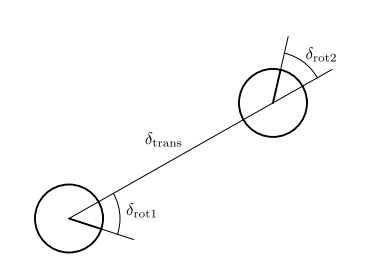
\includegraphics[width=0.6\textwidth]{billeder/odometry}
\caption{Odometry based motion model}
\label{fig:odometry}
\end{figure}
The algorithm for odometry is seen in figure \ref{fig:odometryalgo}. It fits neatly with the way odometry is seen in figure \ref{fig:odometry}.
\begin{figure}[H]
\centering
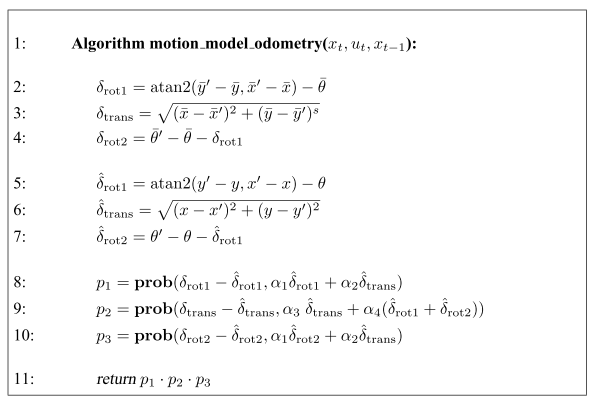
\includegraphics[width=0.8\textwidth]{billeder/odometryalgo}
\caption{Odometry based motion model algorithm}
\label{fig:odometryalgo}
\end{figure}


\subsection{Map based motion model}
Map based motion models seek to incorporate a map in the posterior distribution seen in figure \ref{eq:posterior}. This is done when the map contains relevant information that leads to the following equation:
\begin{equation}
p(x_t | u_t,x_{t-1}) \neq p(x_t | u_t,x_{t-1},m)
\end{equation}
Calculating the map based motion model is a complex task as it needs to incorporate the probability of a path existing in the first place. In order to simplify, we assume that the distance between $x_t$ and $x_{t-1}$ is smaller than half  of the robots diameter. The approximation becomes:
\begin{equation}
p(x_t | u_t,x_{t-1},m) = \eta p(x_t | u_t,x_{t-1})p(x_t|m)
\end{equation}
$\eta$ is the normaliser and $p(x_t|m)$ tells us if it is possible for the robot to even be in that location. An example is seen in figure \ref{fig:mapbased}. For (a)  we assume that we end up somewhere along the black arch. What we do not know is that there is a wall there. When we incorporate the map in (b) we see that for all areas in and around the wall, $p(x_t|m) = 0$.
\begin{figure}[H]
\centering
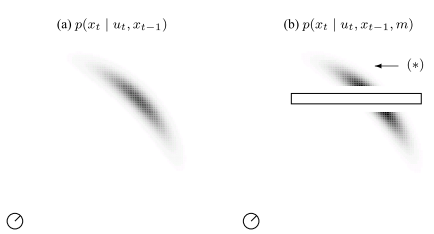
\includegraphics[width=0.8\textwidth]{billeder/mapbased}
\caption{Map based motion model}
\label{fig:mapbased}
\end{figure}

\section{Search and Planning}
The purpose of search and planning is to find the optimal path to the goal. This is done in a discrete environment where you have multiple factors in play. Some of these factors are map, locations \& obstacles and cost. Locations \& obstacles are placed in the map according to their position in the real world. These items will stand in way of our route planning, so we will have to find a way around them. This is illustrated as a matrix below:
\[
\begin{bmatrix}
S & 1 & 0 & 0 & 0\\ 
0 & 1 & 0 & 0 & 0\\ 
0 & 1 & 0 & 0 & 0\\ 
0 & 0 & 0 & 1 & 0\\ 
0 & 0 & 0 & 1 & G
\end{bmatrix}
\]
Ones correspond to obstacles and zeros to cells where we can traverse. S is the start position and G is the Goal.\\
Searching for a path to the goal is done by expanding the cells around the current position. Whenever we expand a cell we also add the cost of moving to that cell to our overall cost value. When we have found our goal, the path with the lowest cost value will be our preferred path.\\
Another example of cost could be if you have a vehicle and were driving through rush hour. The cost of taking left turns would be higher than right turns. This is incorporated into the cost function when searching for a path.\\

\subsection{A\text{*}}
A\text{*} or A star is way to find the shortest path without expanding every cell in our map. This is done with a Heuristic function (called h). The value of the cells in the Heuristic function is added to the cost when expanding cells, $f = h + g$ with g being the cost. The path with the lowest f value is our preferred path. There is one condition that must be true for the Heuristic function as seen below:
\begin{equation}
h(x,y)\leq$ Actual distance $
\end{equation}
The Heuristic function is an approximation of the cost from each cell to the goal without obstacles. An example can be seen below:
\[
\begin{bmatrix}
8 & 7 & 6 & 5 & 4\\ 
7 & 6 & 5 & 4 & 3\\ 
6 & 5 & 4 & 3 & 2\\ 
5 & 4 & 3 & 2 & 1\\ 
4 & 3 & 2 & 1 & 0
\end{bmatrix}
\]
When simulating with A\text{*} it becomes apparent that A\text{*} seeks to expand straight to the goal.

\subsection{Dynamic Programming}
Another way to plan is to use dynamic programming. When searching for the path to the goal, every spot is expanded and a policy is added to the cells. The policy is the optimal action to perform when in that cell. Actions could be to go up, down, left or right in the matrix. An example matrix is seen below: 
\[
\begin{bmatrix}
S & 1 & \downarrow & \downarrow & \downarrow\\ 
\downarrow & 1 & \downarrow & \downarrow & \downarrow\\ 
\downarrow & 1 & \rightarrow & \rightarrow & \downarrow\\ 
\rightarrow & \rightarrow & \uparrow & 1 & \downarrow\\ 
\rightarrow & \rightarrow & \uparrow & 1 & G
\end{bmatrix}
\]
Dynamic programming is useful if the robot deviates from a set path and ends up in another location. The best policy is determined by starting at the goal and going backwards. 


%------------------------------------------------